\subsection{Fitting pipeline}
\todo[inline]{clean this up so this fits into implementation}
\begin{figure}
\centering
  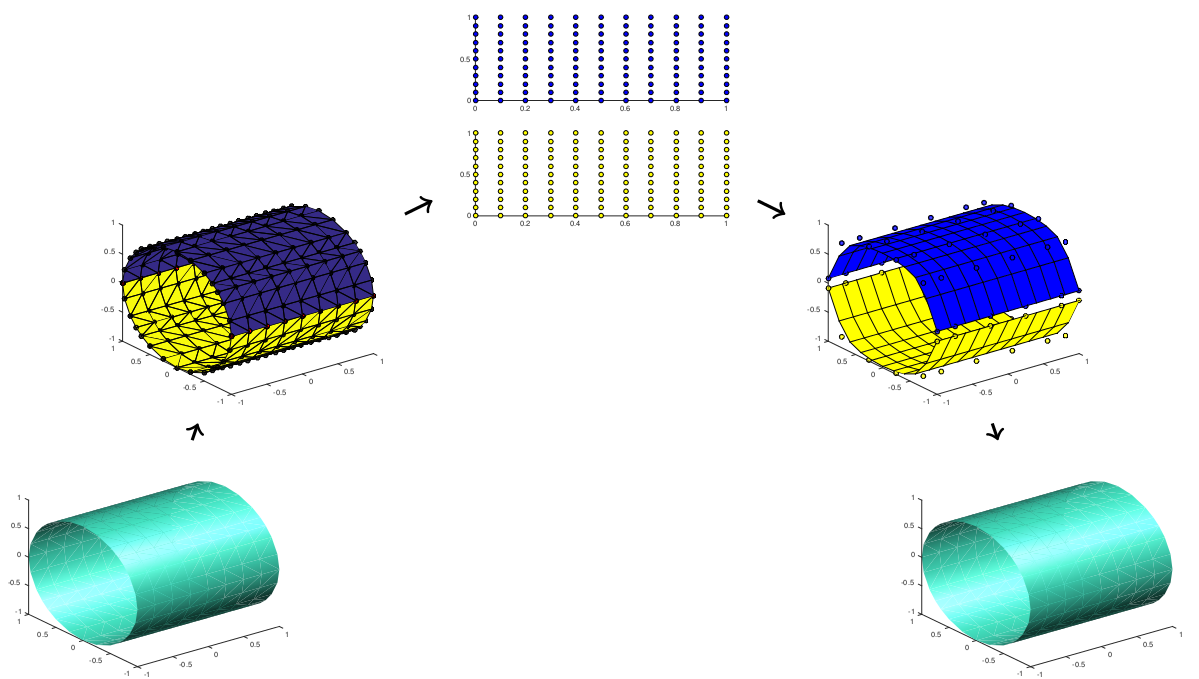
\includegraphics[width=.85\linewidth]{Fitting_workflow.png}
  \caption{NURBS fitting pipeline}
  \label{fig:fitting_pipeline}
\end{figure}
Since the geometry obtained after topology optimization can be arbitrary complex, we might not be able to find a good fit using only one patch. We seek a multi step algorithm, allowing us to break the overall big problem into smaller problems, which can be handled relatively easy.
Based on the algorithm described in \cite{eck1996automatic}, our overall fitting pipeline looks as follows (see \autoref{fig:fitting_pipeline}):
\begin{itemize}
	\item Patch selection (breaking our problem in small pieces which can be solved using least squares)
	\item Parametrization of obtained patches
	\item B-spline fitting using least squares
	\item Smooth connection of patches
	\item Conversion back to CAD
\end{itemize}

The pipeline given above, once implemented, will provide us with a flexible algorithm for converting an arbitrary complex mesh based geometry into NURBS and, hence, CAD-representation.